\begin{frame}{Escoger un lenguaje}
  \begin{center}
    \begin{tabular}{c c c c}
      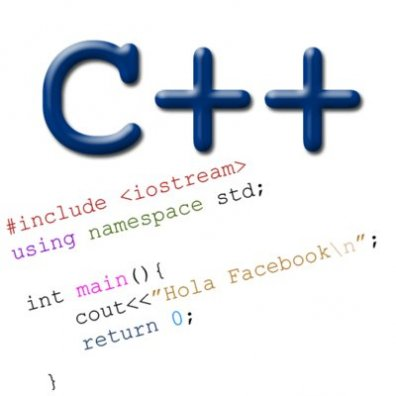
\includegraphics[scale=0.1]{img/cpp} & \pause
      
\includegraphics[scale=0.15]{img/java} & \pause
      
\includegraphics[scale=0.15]{img/haskell} & \pause
      
\includegraphics[scale=0.1]{img/erlang} \\

      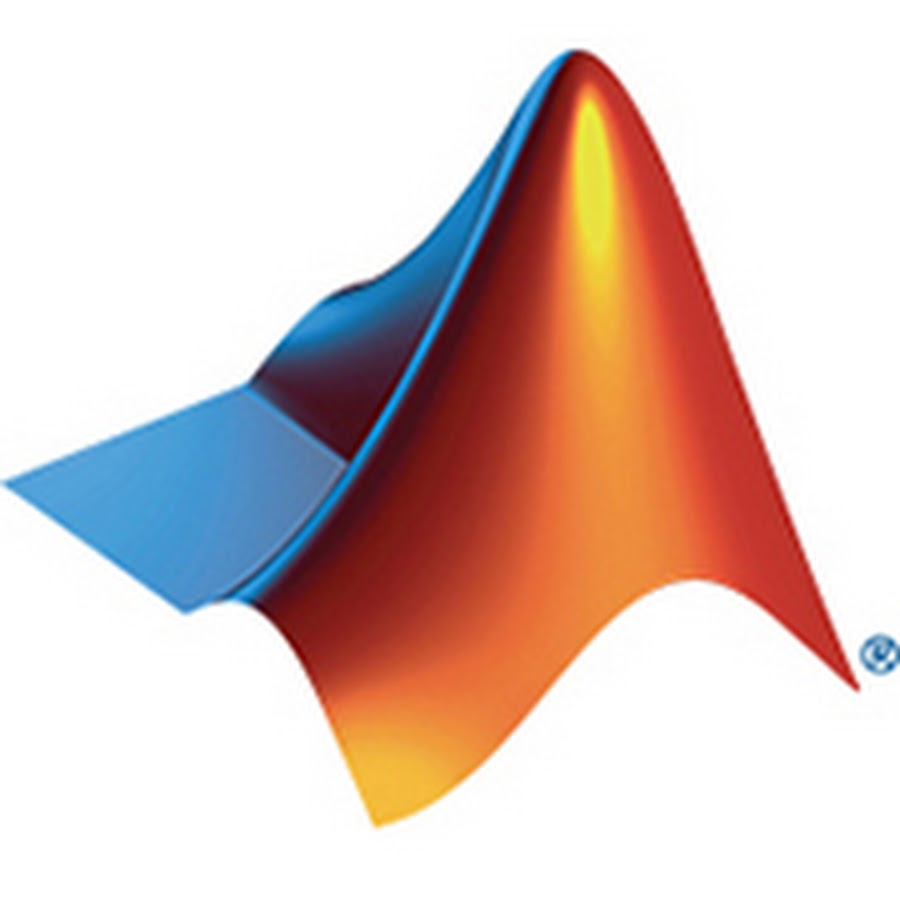
\includegraphics[scale=0.05]{img/matlab} &
      
\includegraphics[scale=0.05]{img/pascal} &
      
\includegraphics[scale=0.15]{img/prolog} &
      
\includegraphics[scale=0.1]{img/smalltalk} \\
    \end{tabular}

    
\includegraphics[scale=0.3]{img/choose_ed}
  \end{center}
\end{frame}

\begin{frame}{Comunicación con la base de datos}
  \begin{itemize}
    \item sqlapi \pause $\rightarrow$ GCC. \pause
    \item MySQL connector \pause $\rightarrow$ ED quiere PostgreSQL. \pause
    \item libodbc \pause $\rightarrow$ Aún en desarrollo. \pause
    \item libpqxx.
  \end{itemize}
\end{frame}

\begin{frame}{Interfaz gráfica}
  \begin{itemize}
    \item Qt.
    \item gtkmm.
    \item wxWidgets.
    \item FLTK.
  \end{itemize}
\end{frame}

\begin{frame}{Diseño estructural}
  Implementar diseño en capas:
  \begin{itemize}
    \item Modelo $\rightarrow$ Encapsular llamadas a DB.
    \item Controlador $\rightarrow$ Crear puentes de comunicación.
    \item Vista $\rightarrow$ Comunicar con librería gráfica.
    \item Debe haber total separación.
  \end{itemize}

  \begin{center}
    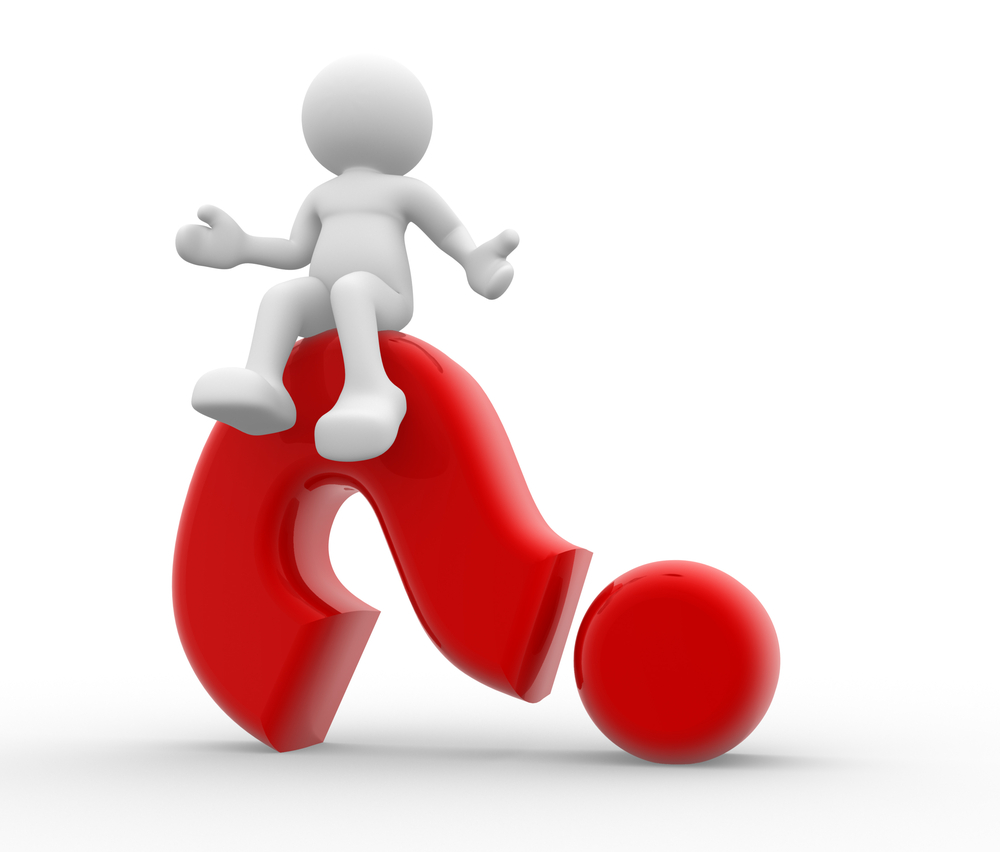
\includegraphics[scale=0.5]{img/ed_realization}
  \end{center}
\end{frame}
